% !TEX encoding = UTF-8 Unicode
%!TEX root = main.tex
% !TEX spellcheck = en-US
%%=========================================


%%%%%%%%%%%%%%%%%%%%%%%%%%%%%%%%%%%%%%%%%%%%%%%%%%%%%%%%%%%%%%%%%%%%%%%%%%%%%%%%%%%
\chapter{Design and Implementation}
\label{ch:design_implementation}
% each feature/

This chapter describes in detail the design and implementation of ProXC++. This includes the runtime data structures used by the scheduler, and how the library features interact with the scheduler and the runtime environment.

Note that the focus of this design and implementation is dynamic multithreading and multicore support. Features and details that has not much relevance to multithreading, such as replicators and C++ syntax, is detailed to a lesser extent.

The library is written in C++, with standard C++14 dialect. The reader is expected to have a fair understanding of C++, and being familiar with standard C++11 dialect or newer is recommended. Detailed explanations of the C++ programming language is not presented here. Refer to any C++ reference (e.g. \citet{stroustrup2013c++}) for more details.


%%%%%%%%%%%%%%%%%%%%%%%%%%%%%%%%%%%%%%%%%%%%%%%%%%%%%%%%%%%%%%%%%%%%%%%%%%%%%%%%
\section{Data Structures}
% intrusive containers
% concurrent queues
% spinlocks


A set of data structures is commonly used by the runtime system. Apart from the C++ Standard Template Library (STL), the most notable data structures are \textit{intrusive containers}, \textit{concurrent queues}, and \textit{mutual exclusion locks}.

Intrusive containers, just as any other containers, stores some kind of data in some sort of way. The difference is how the container stores the necessary data used to organize the data. A non\hyp{}intrusive container is responsible for storing the necessary data, while for an intrusive container the elements are responsible for storing the necessary data. In other words, the element becomes ``aware'' of being a part of the intrusive container. Usually, intrusive containers are implemented with the elements having \textit{hooks} as data members. These hooks contains all the necessary data used by the intrusive container to store the elements. Intrusive containers offers better performance compared to non\hyp{}intrusive containers, as they minimize memory allocations and better memory locality.

Concurrent queues are queues which are safe to use concurrently, often denoted as \textit{thread safe}. The most common approach is taking a non\hyp{}thread safe queue and enforcing mutual exclusion around the critical regions. This approach however is not desirable, as it has very low throughput in multiprogrammed programs. Plenty of research \citep[e.g.][]{chase2005dynamic,le2013correct} has been devoted to creating non\hyp{}blocking queues (see \cref{sec:nonblocking_algorithms}) both available and efficient. Concurrent queues often differentiate between single or multiple producers and consumers. Producers are processes which insert elements into the queue, and consumers are processes which remove elements from the queue. The runtime system uses the variants \textit{single\hyp{}producer\hyp{}multiple\hyp{}consumer} (SPMC) queues and \textit{multiple\hyp{}producer\hyp{}single\hyp{}consumer} (MPSC) queues.

Creating a complete non\hyp{}blocking system is most of the times impossible for a multiprogrammed programs. Sometimes resorting to mutual exclusion in critical regions is unavoidable. Different types of locks is suitable for different situations. Whether the lock is often contested, meaning multiple kernel\hyp{}threads are trying to acquire the lock simultaneously, and if the lock is held for a longer period of time or not, will affect the performance. \Citet[page 196--199]{brown2007c++csp2} performs a case study on different mutexes, describing various mutex algorithms and provides a benchmark and analysis of their performance. The conclusion from the case study is that for low contested, short\hyp{}term held mutexes, spinlocks yields best performance regarding low latency. 

For multiprocessor architectures, the \textit{test\hyp{}and\hyp{}test\hyp{}and\hyp{}set} (TTAS) spinlock is generally favorable as it causes less memory contention than the standard spinlock. Instead of constantly trying to test\hyp{}and\hyp{}set the lock, it waits until the lock appears free. Different variants of the TTAS spinlock includes constant/exponential backoff during contention and cache friendly atomic operations.


\FloatBarrier
%%%%%%%%%%%%%%%%%%%%%%%%%%%%%%%%%%%%%%%%%%%%%%%%%%%%%%%%%%%%%%%%%%%%%%%%%%%%%%%%
\section{Runtime System Overview}
\label{sec:runtime_system_overview}

The runtime system for ProXC++ is based on \textit{contexts}, which represent a point of computational execution. A context is a user\hyp{}thread, meaning it has its own program stack and processor context. A kernel\hyp{}thread always has a main context and a scheduler context, while it may have zero or more work contexts. Contexts are based on the hybrid threading model (see \cref{subsec:threading_models}).

At startup, the initial main context creates $N-1$ kernel\hyp{}threads, given the processor has $N$ online logical cores. Each main context then creates a scheduler context, which represent the runtime environment for each kernel\hyp{}thread. Only the initial main context does any meaningful work, as the other main contexts only purpose is to spawn and join the scheduler context. Whenever the initial main context returns, the runtime environment will cleanup and shutdown. At the creation of a new kernel\hyp{}thread, along side with its main context and scheduler context, the scheduler will wait as idle (block) until available work is ready in other schedulers.

\Cref{fig:runtime_overview} displays a rough outline of how the contexts, user\hyp{}threads and kernel\hyp{}threads are organized relative to each other. Note that even though work contexts are present in each kernel\hyp{}thread, it 

\begin{figure}[h!]
    \centering
    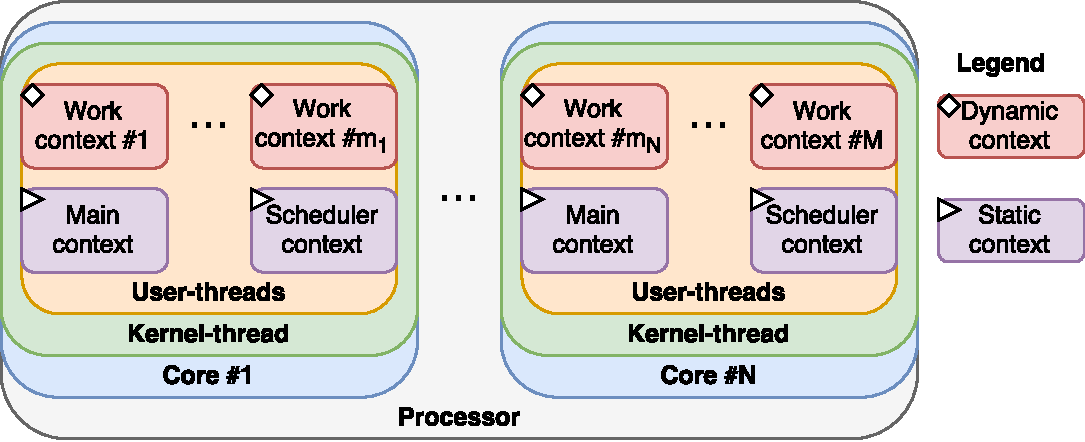
\includegraphics[width=0.8\linewidth]{fig/runtime_overview}
    \caption{Overview of the runtime system, with N online processor cores.}
    \label{fig:runtime_overview}
\end{figure}

Work is distributed among schedulers through work stealing (see \cref{subsec:work_stealing}). This is achieved by each scheduler having a double\hyp{}ended queue (deque for short) containing ready work for that given scheduler. Whenever work is spawned by a scheduler, or idle work becomes ready, it is pushed onto the deque. This allows idle schedulers to try steal work and resume.


\FloatBarrier
%%%%%%%%%%%%%%%%%%%%%%%%%%%%%%%%%%%%%%%%%%%%%%%%%%%%%%%%%%%%%%%%%%%%%%%%%%%%%%%%
\subsection{Contexts}
\label{subsec:contexts}

The runtime system differentiates contexts in two categories: \textit{process vs. scheduler} and \textit{static vs. dynamic}.

A process context represents a part of computation from the program, while the scheduler context is, as the name implies, the scheduler which is in control of scheduling the different process contexts. A static context is a context which cannot \textit{migrate} between schedulers, while a dynamic context can.

For every kernel\hyp{}thread, there always exist a \textit{main context} and a \textit{scheduler context}. The main context is the context of the actual kernel\hyp{}thread, meaning the kernel\hyp{}thread returns when the main context returns. It is a process context, since it represents a part of the computation in the program, and a static context, since it cannot migrate between schedulers. It is undefined behaviour FIXME for main context to return (exit) on a kernel\hyp{}thread different from where it originated from, which is why the main context is static.

The scheduler context is responsible for creating new work contexts, schedule between work contexts, and destroying finished work contexts. The scheduler is never visible to the programmer, and is the driving force behind the runtime environment. The scheduler is obviously a static context, as having multiple schedulers on the same kernel\hyp{}thread is unintuitive and unproductive.

Besides the main and scheduler context, the rest of the program is composed by \textit{work contexts}. Work contexts are process contexts, but opposed to the main context, are dynamic instead of static. Being dynamic allows work contexts to migrate between schedulers. 

Contexts are implemented using the Boost Context library \citep{kowalke2017boost}. Boost Context creates an abstraction over the execution state of a thread called \textit{execution context}, which includes stack and stack pointer, local variables, CPU registers and flags, and instruction pointer. The execution context allows transfer of control between other execution contexts, allowing to build higher level abstractions such as user\hyp{}threads. Execution contexts can also migrate between kernel\hyp{}threads.

The context data structure is represented as a class, containing an execution context as well as a collection of flags, intrusive hooks, a wait queue, and a spinlock. The context class only acts as an information container for a given user\hyp{}thread, as most of the functionality of the context is implemented by the scheduler.


%%%%%%%%%%%%%%%%%%%%%%%%%%%%%%%%%%%%%%%%%%%%%%%%%%%%%%%%%%%%%%%%%%%%%%%%%%%%%%%%
\subsection{Processes}
\label{subsec:processes}

A concurrent program using ProXC++ consists of \textit{processes}, called \textit{proc} in code. These processes, same as in CSP, are independent points of execution, with each running sequential code. In code, a process is represented by a function and its corresponding arguments. When scheduled, the function is executed concurrently with the rest of the program, and exits when the function returns. 

The process is no more than an opaque type to a context. The programmer implicitly creates new contexts through processes, while the scheduler under the hood operates on the contexts.

Processes can be dynamically generated, either through explicitly creating a dynamic collection of processes or through use of replicators.


%%%%%%%%%%%%%%%%%%%%%%%%%%%%%%%%%%%%%%%%%%%%%%%%%%%%%%%%%%%%%%%%%%%%%%%%%%%%%%%%
\subsection{Scheduler}
\label{subsec:scheduler}
% work stealing
% process create, schedule, join, destroy
% process timeouts

The scheduler is the corner piece of runtime system. It has the sole responsibility of managing the different contexts, including creating, scheduling, destroying contexts. The scheduler runs as its own context, running in an scheduler loop until the program exits. Each spawned kernel\hyp{}thread contains a scheduler context, and the scheduler context never migrates to an another kernel\hyp{}thread. Each scheduler is the ``owner'' of one or more process contexts. ``Owning'' a context is synonymous with management, involving scheduling, inter\hyp{}process handling, and destroying the context when exited. When a process is created, the scheduler residing on the same kernel\hyp{}thread ``owns'' that context. Only one scheduler can ``own'' a context at a time.

Each scheduler contains four queues, namely a work, sleep, terminated, and remote queue. The work, sleep and terminated queue is managed only by a single scheduler, and is used to organize the processes the scheduler ``owns''. The work and terminated queues are intrusive doubly linked lists, while the sleep queue is a sorted, intrusive multiset. The work queue is the total list of all processes the scheduler ``own''. The sleep queue contains all process which are suspended with a given timeout, and are sorted in ascending order. The terminated queue is the queue of all processes which has terminated. The need for this queue will be explained later. 

The remote queue is a concurrent MPSC queue, where the managing scheduler is the consumer while any other schedulers are the producer. Whenever a scheduler readies a context and it does not ``own'' it, the context is placed in the remote queue to the ``owning'' scheduler. The ``owning'' scheduler transitions contexts in the remote queue to the ready queue. In essence, the remote queue is used to signal schedulers when their contexts are readied, since remote schedulers cannot safely access the ready queue.




%%%%%%%%%%%%%%%%%%%%%%%%%%%%%%%%%%%%%%%%%%%%%%%%%%%%%%%%%%%%%%%%%%%%%%%%%%%%%%%%
\section{Parallel}



\section{Timers}



\section{Channels}




\section{Alt}

